\documentclass[a4paper, 14pt]{extarticle}
\usepackage[russian]{babel}
\usepackage[T1]{fontenc}
\usepackage{fontspec}
\usepackage{indentfirst}
\usepackage{enumitem}
\usepackage{graphicx}
\usepackage[
  left=20mm,
  right=10mm,
  top=20mm,
  bottom=20mm
]{geometry}
\usepackage{parskip}
\usepackage{titlesec}
\usepackage{xurl}
\usepackage{hyperref}
\usepackage{float}
\usepackage[
  figurename=Рисунок,
  labelsep=endash,
]{caption}
\usepackage[outputdir=build, newfloat]{minted}

\hypersetup{
  colorlinks=true,
  linkcolor=black,
  filecolor=blue,
  urlcolor=blue,
}

\renewcommand*{\labelitemi}{---}
\setmainfont{Times New Roman}
\setmonofont{JetBrains Mono}[
  SizeFeatures={Size=11},
]

\newenvironment{code}{\captionsetup{type=listing}}{}
\SetupFloatingEnvironment{listing}{name=Листинг}

\setminted{
  fontsize=\footnotesize,
  frame=lines,
  framesep=2mm,
}

\setlength{\parskip}{6pt}

\setlength{\parindent}{1cm}
\setlist[itemize]{itemsep=0em,topsep=0em,parsep=0em,partopsep=0em,leftmargin=2.0cm,wide}
\setlist[enumerate]{itemsep=0em,topsep=0em,parsep=0em,partopsep=0em,leftmargin=2.0cm,wide}

\renewcommand{\thesection}{\arabic{section}.}
\renewcommand{\thesubsection}{\thesection\arabic{subsection}.}
\renewcommand{\thesubsubsection}{\thesubsection\arabic{subsubsection}.}

\titleformat{\section}{\normalfont\bfseries}{\thesection}{0.5em}{}
\titleformat{\subsection}{\normalfont\bfseries}{\thesubsection}{0.5em}{}

\titleformat*{\section}{\normalfont\bfseries}
\titleformat*{\subsection}{\normalfont\bfseries}

\linespread{1.5}
\renewcommand{\baselinestretch}{1.5}

\begin{document}

\begin{titlepage}
  \vspace{0pt plus2fill}
  \noindent

  \vspace{0pt plus6fill}
  \begin{center}
    Санкт-Петербургский национальный исследовательский университет
    информационных технологий, механики и оптики

    \vspace{0pt plus3fill}

    Факультет инфокоммуникационных технологий

    Направление подготовки 11.03.02

    \vspace{0pt plus2fill}

    Лабораторная работа №1

    <<Работа с заметками>>

  \end{center}

  \vspace{0pt plus6fill}
  \begin{flushright}
    Выполнил: \\
    Швалов Даниил Андреевич

    Группа: К33211

    Проверила: \\
    Марченко Елена Вадимовна
  \end{flushright}

  \vspace{0pt plus5fill}
  \begin{center}
    Санкт-Петербург

    2024
  \end{center}
\end{titlepage}

\section{Введение}

\textbf{Цель работы}: разработать веб-приложение, в котором у пользователя будет
возможность создавать заметки и оставлять комментарии к ним.

В данной лабораторной работе необходимо разработать веб-приложение с заметками.
При этом необходимо сделать так, чтобы последняя добавленная заметка
отображалась в самом верху списка заметок. Также необходимо, чтобы к заметкам
можно было создавать комментарии.

\section{Ход работы}

Для хранения данных приложения была выбрана СУБД PostgreSQL. Данная СУБД
поддерживается в языке программирования PHP и не требует дополнительной
установки внешних библиотек для работы с СУБД. Кроме того, СУБД PostgreSQL
является высокопроизводительным решением, обладающим активным сообществом,
большим количеством документации. Данное решение используется множеством
компаний, поскольку оно зарекомендовало себя как надежное и эффективное
хранилище данных.

На рисунке \ref{fig:puml/database.png} изображена схема таблиц базы данных. В
ней представлены две таблицы: <<note>> и <<comment>>.

\begin{figure}[H]
  \centering
  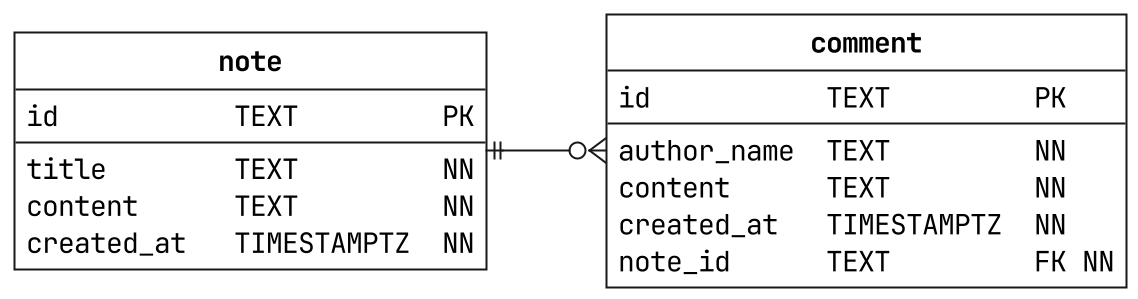
\includegraphics[width=0.8\textwidth]{images/puml/database.png}
  \caption{Схема таблиц базы данных}
  \label{fig:puml/database.png}
\end{figure}

В таблице <<note>> хранится информация о заметках: заголовок заметки, ее
содержимое и дата создания. Дата создания используется для сортировки заметок
при показе пользователю.

В таблице <<comment>> хранится информация о комментариях к заметке. В ней есть
такие столбцы, как имя автора, содержимое комментария, дата создания
комментария, а также идентификатор заметки. В данном  случае дата создания также
используется для сортировки комментариев.

На рисунке \ref{fig:notes.png} представлена страница, которая встречает
пользователя при открытии веб-приложения. На ней пользователь может открыть одну
доступных из заметок или создать свою, нажав на кнопку <<Создать заметку>>.
Заметки, отображаемые пользователю, отсортированы в порядке убывания: от самых
новых к самым старым.

\begin{figure}[H]
  \centering
  \fbox{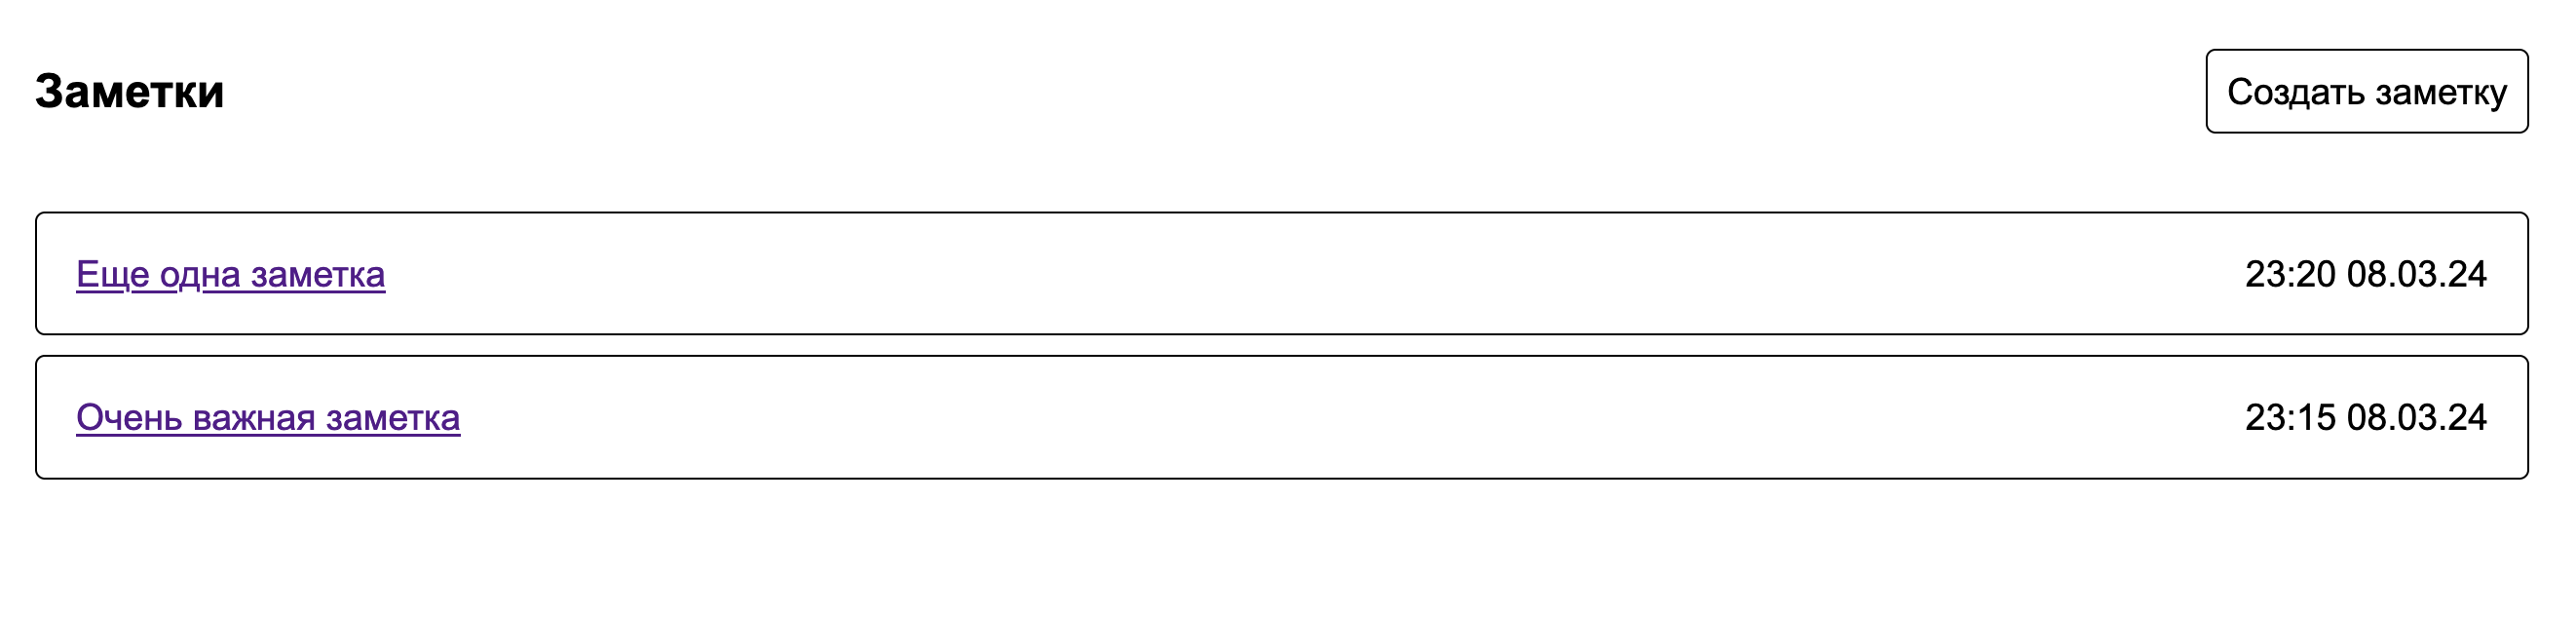
\includegraphics[width=\textwidth]{images/notes.png}}
  \caption{Страница с заметками}
  \label{fig:notes.png}
\end{figure}

При создании заметки пользователю открывается форма, показанная на рисунке
\ref{fig:note-form.png}. На ней пользователю предлагается ввести заголовок и
содержимое заметки.

\begin{figure}[H]
  \centering
  \fbox{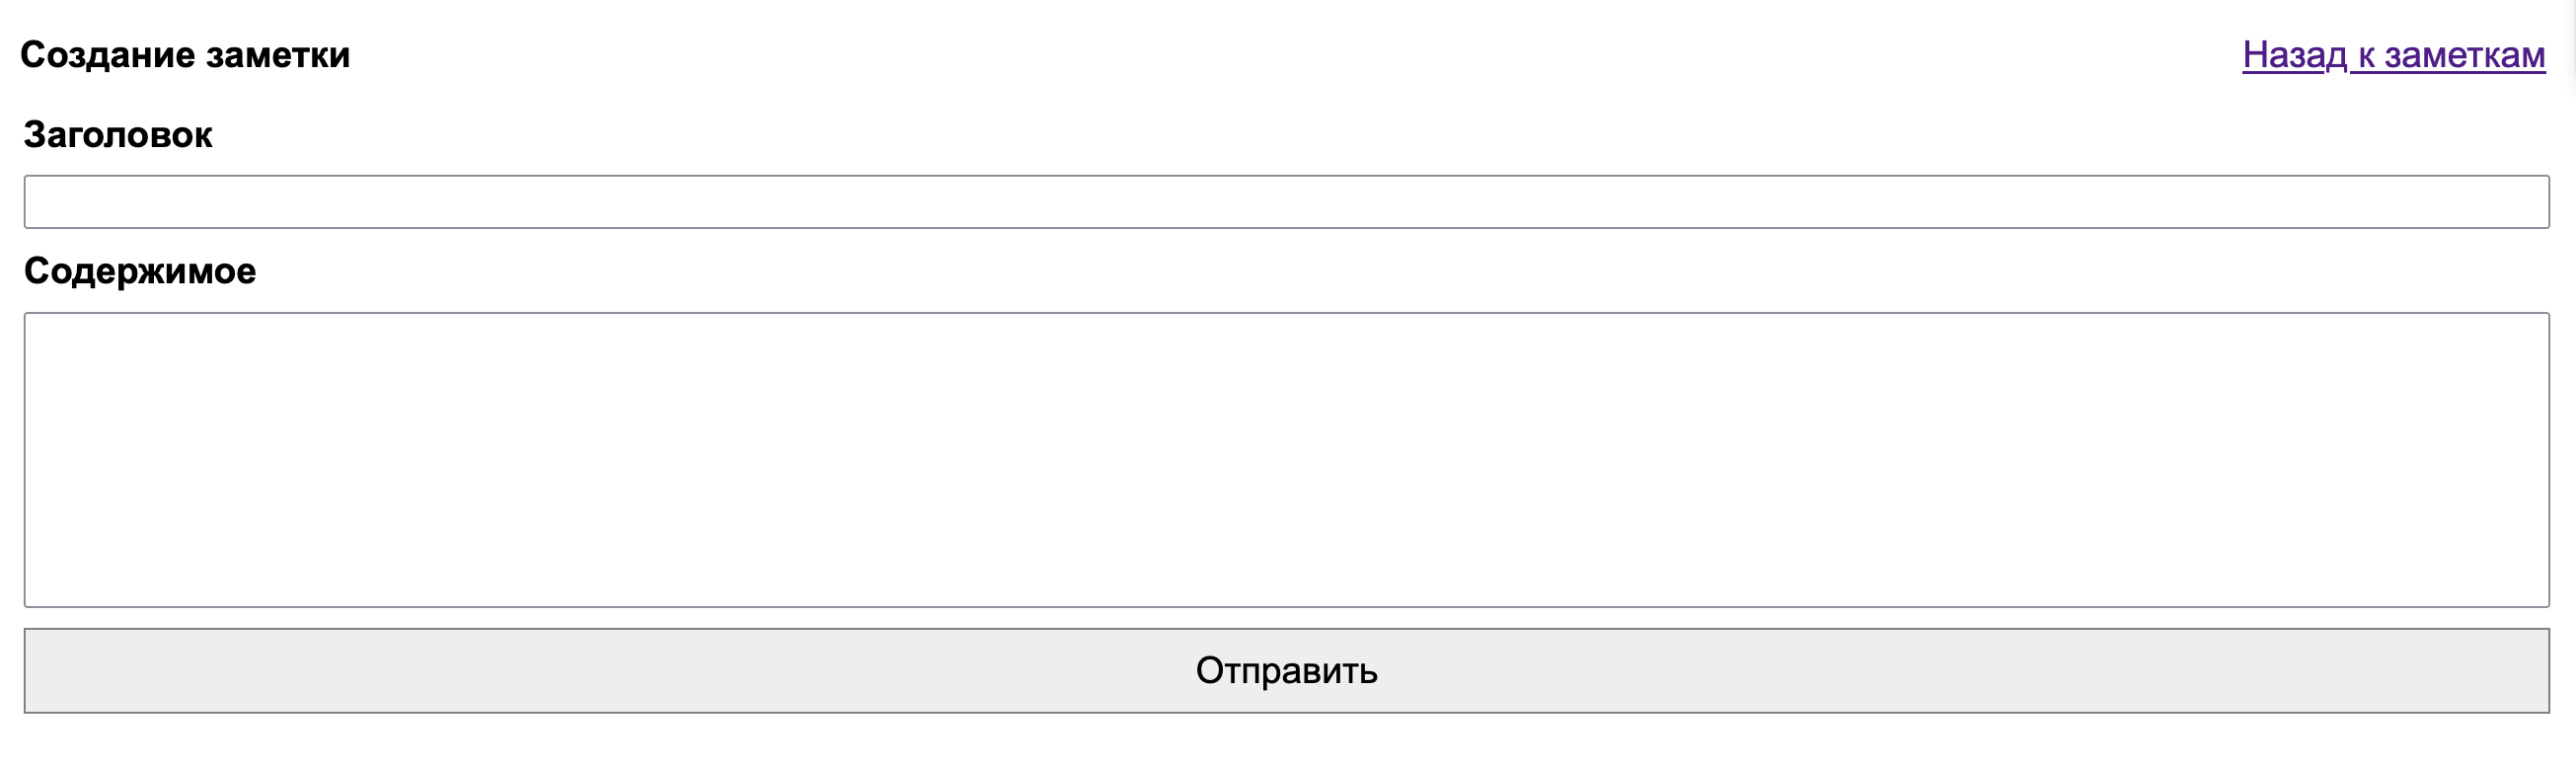
\includegraphics[width=\textwidth]{images/note-form.png}}
  \caption{Страница с созданием заметки}
  \label{fig:note-form.png}
\end{figure}

При открытии заметки пользователю показывается страница, изображенная на рисунке
\ref{fig:note.png}. На ней пользователь видит заголовок заметки, ее содержимое,
а также форму для создания комментариев. Комментарии сортируются в порядке
убывания: от самых новых к самым старым.

\begin{figure}[H]
  \centering
  \fbox{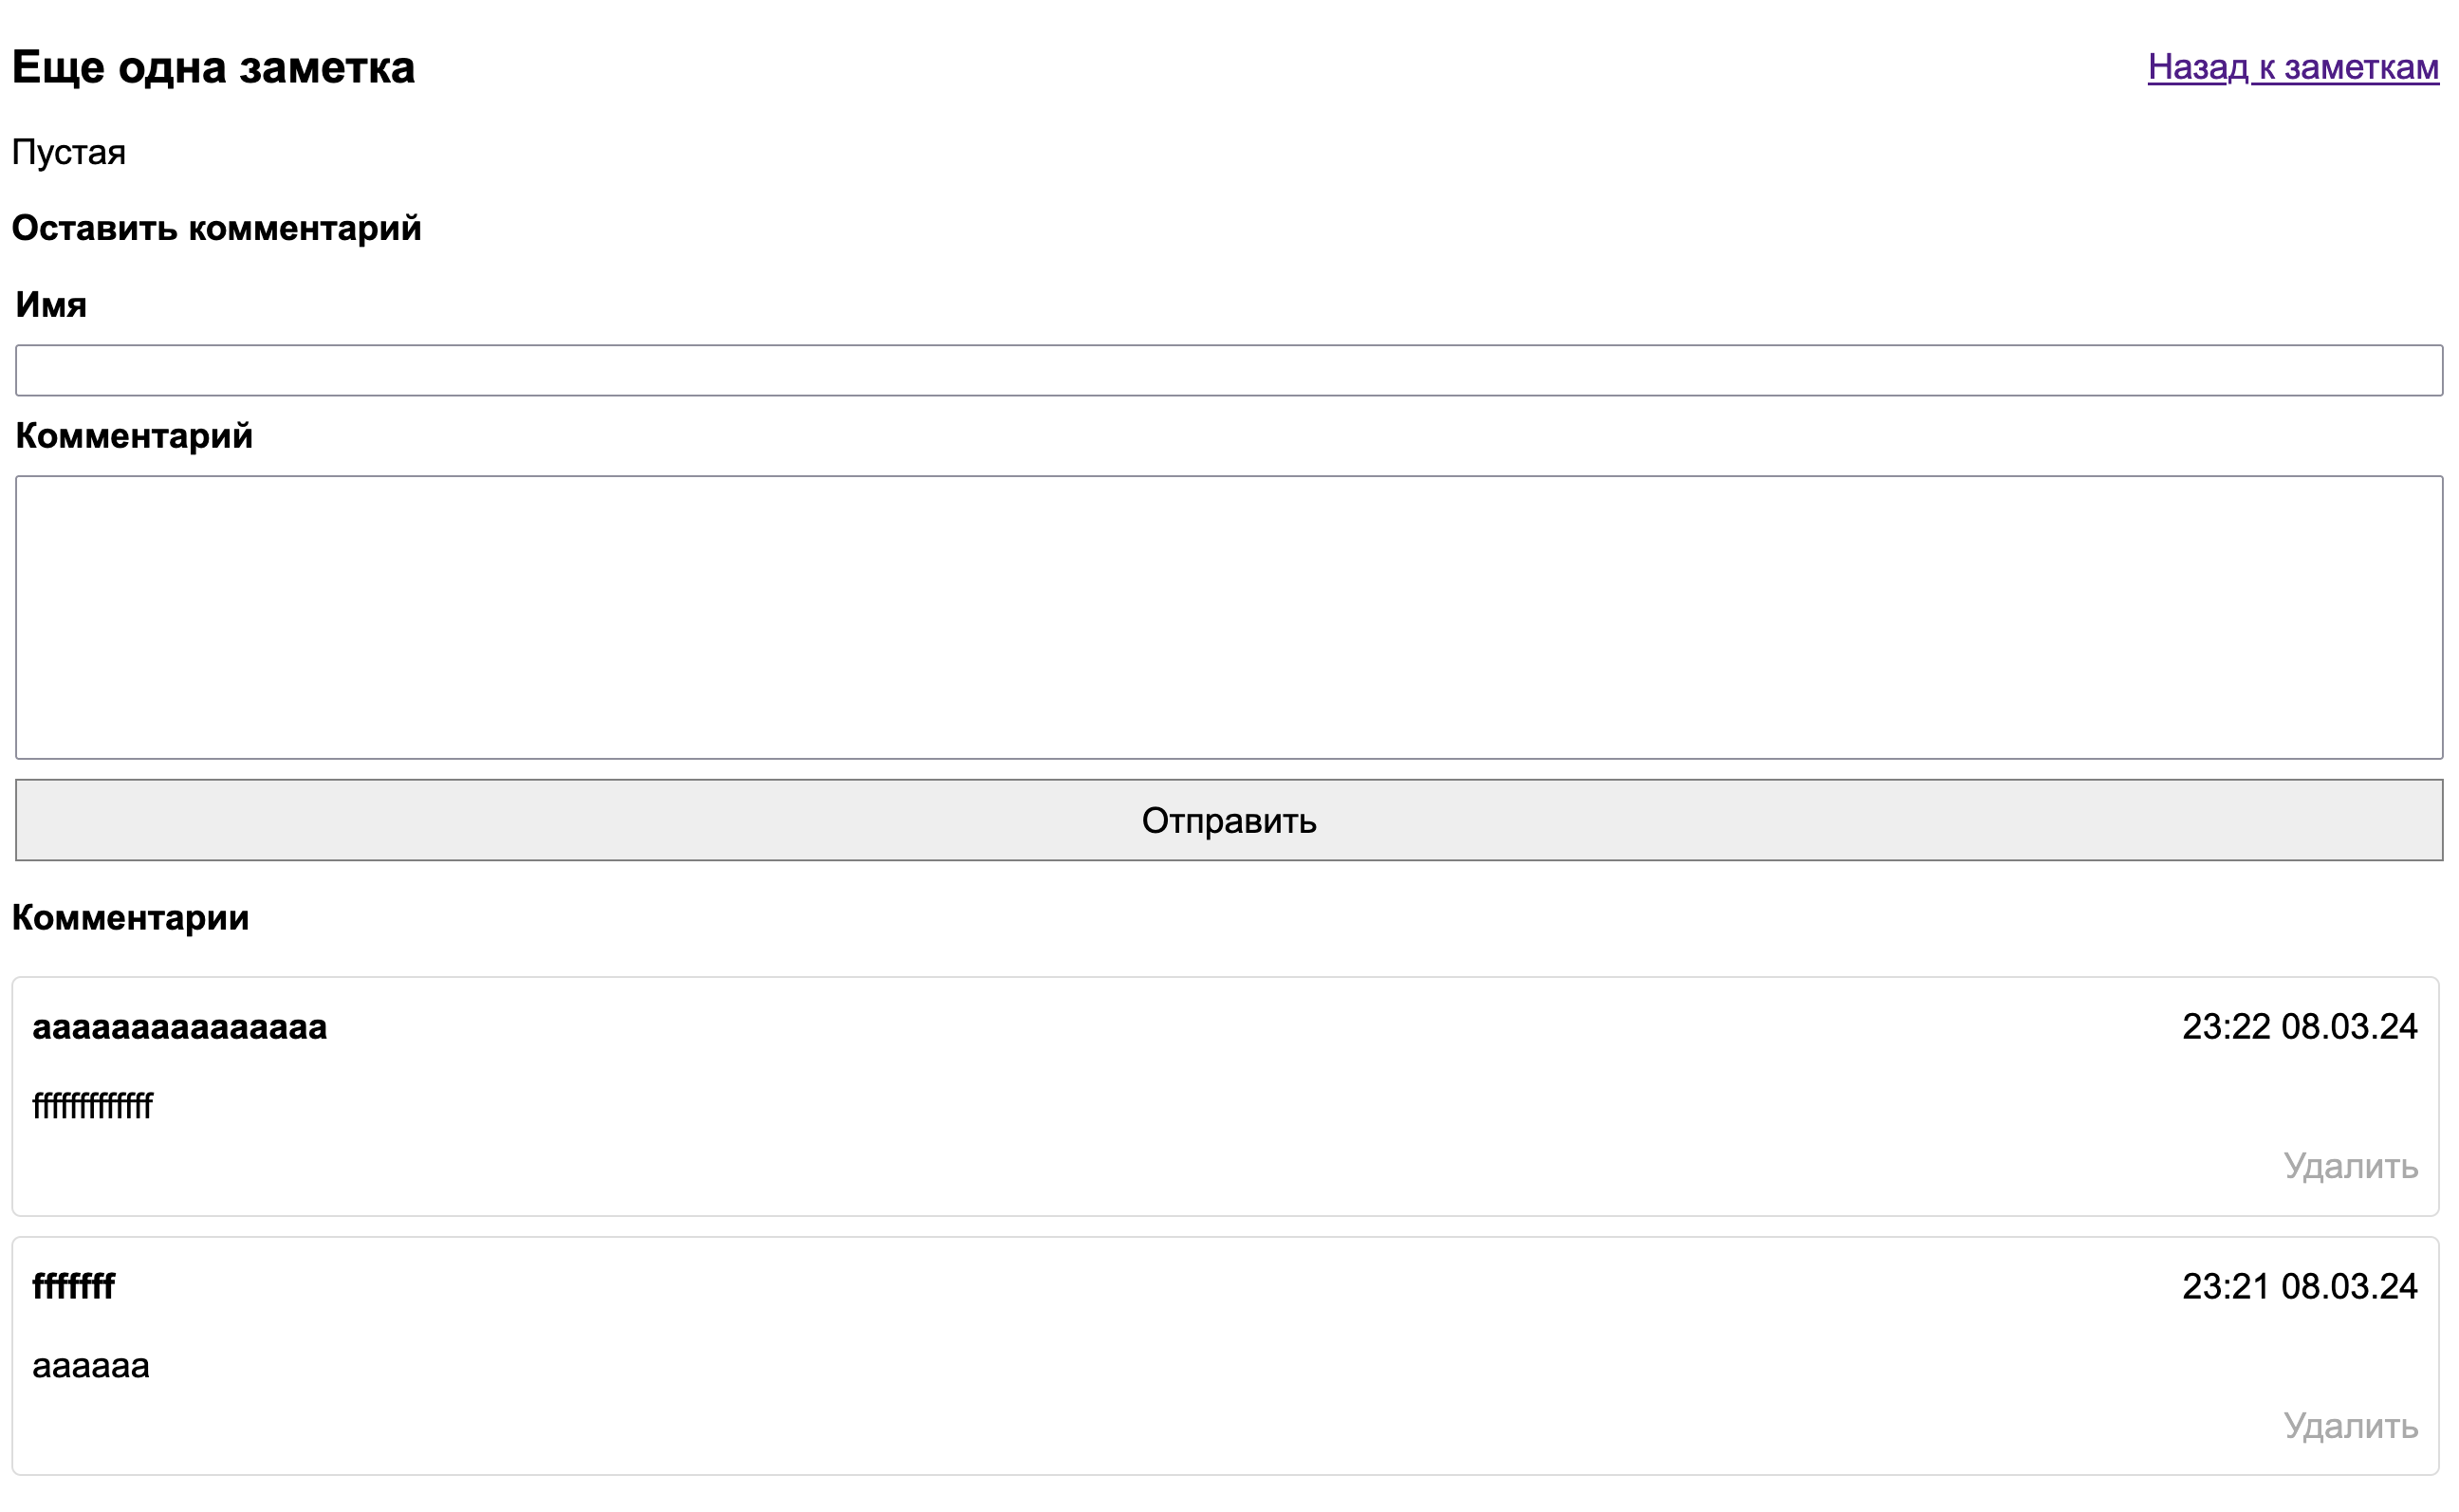
\includegraphics[width=\textwidth]{images/note.png}}
  \caption{Страница с содержимым заметки и комментариями}
  \label{fig:note.png}
\end{figure}

\section{Вывод}

В ходе выполнения лабораторной работы было разработано веб-приложение, в котором
у пользователя есть возможность создавать заметки и оставлять комментарии к ним.

\end{document}
